\documentclass[10pt]{article}
\usepackage[a4paper, margin=2cm]{geometry}
%\usepackage{fullpage}
\usepackage[T1]{fontenc}
\usepackage[utf8]{inputenc}
\usepackage{graphicx}
\usepackage{mathpazo}
\pagenumbering{arabic}
\usepackage{siunitx}
\usepackage{amsmath}
\usepackage{mathtools} % Para poder usar "\Aboxed"
\usepackage{cancel} % Para usar "\cancel", de https://tex.stackexchange.com/questions/537955/how-do-cross-out-text-in-math-mode
\usepackage{multicol}
\usepackage[spanish]{babel}
\usepackage{steinmetz}
\DeclareSIUnit\voltampere{VA}
\DeclareSIUnit\var{VAr}
\setlength\parindent{0pt} % no indent

% Numbering pages on the right footer:
% (https://tex.stackexchange.com/questions/153167/how-to-set-page-number-at-right-footer)
\usepackage{fancyhdr}
% Turn on the style
\pagestyle{fancy}
\fancyhf{} % sets both header and footer to nothing
\renewcommand{\headrulewidth}{0pt} % To remove the top horizontal line created by default by "fancyhdr", from here: https://tex.stackexchange.com/questions/13896/how-to-remove-the-top-horizontal-bar-in-fancyhdr
% Set the right side of the footer to be the page number
\fancyfoot[R]{\thepage}


\usepackage{minibox} % Para poder partir el texto en 2 líneas usando "underbrace" u "overbrace", info aquí: https://tex.stackexchange.com/questions/8680/how-can-i-insert-a-newline-in-a-framebox


\usepackage{xparse} % For "overbrace/underbrace but with an arrow instead", from https://tex.stackexchange.com/questions/8720/overbrace-underbrace-but-with-an-arrow-instead

% Para poner flechas sobre los signos de igual, de aquí: https://tex.stackexchange.com/questions/8720/overbrace-underbrace-but-with-an-arrow-instead
\NewDocumentCommand{\overarrow}{O{=} O{\uparrow} m}{%
  \overset{\makebox[0pt]{\begin{tabular}{@{}c@{}}#3\\[0pt]\ensuremath{#2}\end{tabular}}}{#1}
}
\NewDocumentCommand{\underarrow}{O{=} O{\downarrow} m}{%
  \underset{\makebox[0pt]{\begin{tabular}{@{}c@{}}\ensuremath{#2}\\[0pt]#3\end{tabular}}}{#1}
}



\begin{document}

\large{\textbf{Ejercicio 5 de la colección de problemas}} (modificado para resolver por nudos)

\vspace{3mm}
\large{\textbf{Enunciado}}:

\vspace{3mm}
Analizar el circuito de la figura mediante el método de los nudos, obteniendo el valor de las corrientes de rama.

\begin{minipage}{0.75\linewidth}
  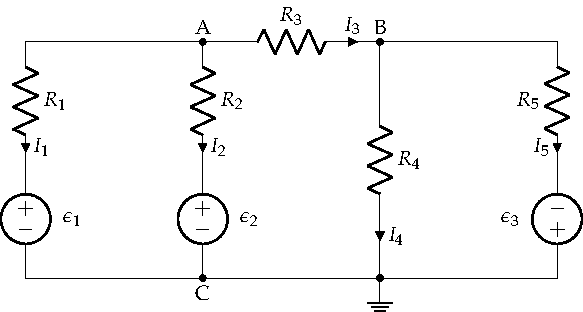
\includegraphics[scale=1.2]{figs/ejercicio5_coleccion_nudos1.pdf}
\end{minipage}
\begin{minipage}{0.25\linewidth}
    \textbf{Datos}:
    \vspace{2mm}
    
    $R_1 = R_2 = \qty{1}{\ohm}$\\ 
    $R_3 = \qty{2}{\ohm}$\\
    $R_4 = \qty{3}{\ohm}$\\
    $R_5=\qty{4}{\ohm}$\\
    $\epsilon_1=\qty{118}{\volt}$\\
    $\epsilon_2 = \qty{236}{\volt}$\\
    $\epsilon_3 = \qty{118}{\volt}$    
\end{minipage}

\vspace{4mm}

\hrulefill

\vspace{5mm}
\textbf{Solución}:
\vspace{4mm}

Hemos elegido el nudo $C$ como referencia de potenciales por ser el que conecta mayor número de elementos.

\vspace{2mm}
Primero, transformamos las fuentes de tensión a fuentes de corriente:

\vspace{2mm}
\begin{minipage}{0.9\linewidth}
  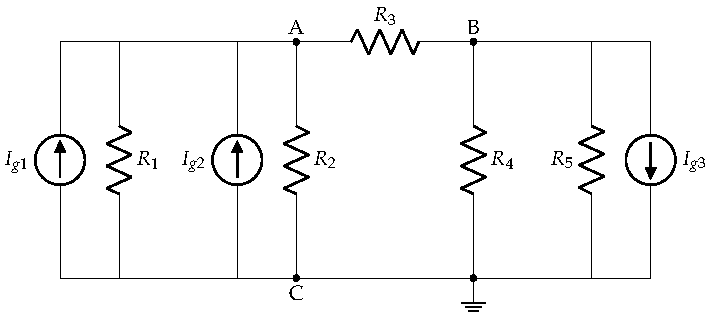
\includegraphics[scale=1.15]{figs/ejercicio5_coleccion_nudos2.pdf}
\end{minipage}
\begin{minipage}{0.1\linewidth}
    Donde:
    \vspace{3mm}
    
    $I_{g_1} = \dfrac{\epsilon_1}{R_1}$\\[6pt]
    $I_{g_2} = \dfrac{\epsilon_2}{R_2}$\\[6pt]   
    $I_{g_3} = \dfrac{\epsilon_3}{R_3}$
\end{minipage}

\vspace{4mm}

Ahora podemos aplicar la ecuación general del método de los nudos:
\begin{equation*}
  \begin{bmatrix}
    G_1 + G_2 + G_3 & -G_3 \\
    -G_3 & G_3 + G_4 + G_5  
  \end{bmatrix}
  \cdot
  \begin{bmatrix}
    U_a\\
    U_b
  \end{bmatrix}
  =
  \begin{bmatrix}
    I_{g_1} + I_{g_2}\\
    -I_{g_3}
  \end{bmatrix}
\end{equation*}
cuya solución es:
\begin{align*}
  U_a &= \qty{150}{\volt}\\
  U_b &= \qty{42}{\volt}
\end{align*}

De este resultado, obtenemos las corrientes de rama, aplicando 2LK:

\begin{align*}
  I_1 &= \frac{U_{AC} - \epsilon_1}{R_1} = \boxed{\qty{32}{\ampere}}\\[6pt]
  I_2 &= \frac{U_{AC} - \epsilon_2}{R_2} = \boxed{\qty{-86}{\ampere}}\\[6pt]
  I_3 &= \frac{U_{AB}}{R_3} = \boxed{\qty{54}{\ampere}}\\[6pt]
  I_4 &= \frac{U_{BC}}{R_4} = \boxed{\qty{14}{\ampere}}\\[6pt]
  I_5 &= \frac{U_{BC} + \epsilon_3}{R_1} = \boxed{\qty{40}{\ampere}}
\end{align*}

\vspace{4mm}

\emph{Se recomienda comprobar que estos resultados cumplen la 1LK} en cada uno de los 2 nudos independientes del \underline{circuito original} (antes de transformar las fuentes de tensión, porque tambien podríais haber cometido errores al transformar las fuentes), para asegurarse de que la resolución es correcta.

\end{document}
